\section{Schroedinger equation in 1d}

We are interested in finding the bound states of 1d time-independent Schroedinger equation:
\begin{equation}
\left[ -\frac{1}{2}\frac{\mathrm{d}^2}{\mathrm{d}x^2} + V(x) \right] \psi(x) = E\, \psi(x)
\label{eq:Sch_1d_eq}
\end{equation}
%
with the boundary conditions:
%
\begin{equation}
\lim_{x \rightarrow \pm \infty} \psi(x) = 0
\label{eq:BC_isolated}
\end{equation}
%
This boundary condition is relavant for non-periodic systems such as atoms and molecules.

\subsection{Grid points}

First we need to define a spatial domain $\left[x_{\mathrm{min}}, x_{\mathrm{max}}\right]$
where $x_{\mathrm{min}}, x_{\mathrm{max}}$ chosen
such that the boundary condition \ref{eq:BC_isolated} is approximately satisfied.
The next step is to divide the spatial domain $x$ using equally-spaced grid points
which we will denote as $\{x_{1},x_{2},\ldots,x_{N}\}$ where $N$ is number
of grid points. Various spatial quantities such as wave functions and potentials will be discretized
on these grid points.
The grid points $x_{i}$, $i = 1, 2, \ldots$ are chosen as:
\begin{equation}
x_{i} = x_{\mathrm{min}} + (i-1)h
\end{equation}
where $h$ is the spacing between the grid points:
\begin{equation}
h = \frac{ x_{\mathrm{max}} - x_{\mathrm{min}} }{N-1}
\end{equation}

The following Julia code can be used to initialize the grid points:
\begin{juliacode}
function init_FD1d_grid( x_min::Float64, x_max::Float64, N::Int64 )
    L = x_max - x_min
    h = L/(N-1) # spacing
    x = zeros(Float64,N) # the grid points
    for i = 1:N
        x[i] = x_min + (i-1)*h
    end
    return x, h
end
\end{juliacode}

\subsection{Approximating second derivative}

Our next task is to find an approximation to the second derivative operator
present in the Equation \eqref{eq:Sch_1d_eq}.
One simple approximation that we can use is the 3-point (central) finite difference:
\begin{equation}
\frac{\mathrm{d}^2}{\mathrm{d}x^2} \psi_{i} \approx
\frac{\psi_{i+1} - 2\psi_{i} + \psi_{i-1}}{h^2}
\end{equation}
where we have the following notation have been used: $\psi_{i} = \psi(x_{i})$.
%
By taking $\{ \psi_{i} \}$ as a column vector, the second derivative operation
can be expressed as matrix multiplication:
\begin{equation}
\vec{\psi''} = \mathbb{D}^{(2)} \vec{\psi}
\end{equation}
%%
where $\mathbb{D}^{(2)}$ is the second derivative matrix operator:
\begin{equation}
\mathbb{D}^{(2)} = \frac{1}{h^2}
\begin{bmatrix}
-2  &  1  &  0  &  0  & 0 & \cdots & 0 \\
 1  & -2  &  1  &  0  & 0 & \cdots & 0 \\
 0  &  1  & -2  &  1  & 0 & \cdots & 0 \\
 \vdots  &  \ddots  &  \ddots  & \ddots  & \ddots  & \ddots & \vdots \\
 0 & \cdots & 0 & 1 & -2 & 1 & 0 \\
 0  &  \cdots  & \cdots & 0  & 1  & -2  & 1 \\
 0  &  \cdots  & \cdots & \cdots & 0  &  1  & -2 \\
\end{bmatrix}
\label{eq:1d_D2_matmul}
\end{equation}

An example implementation can be found in the following function.
\begin{juliacode}
function build_D2_matrix_3pt( N::Int64, h::Float64 )
    mat = zeros(Float64,N,N)
    for i = 1:N-1
        mat[i,i] = -2.0
        mat[i,i+1] = 1.0
        mat[i+1,i] = mat[i,i+1]
    end
    mat[N,N] = -2.0
    return mat/h^2
end
\end{juliacode}


Before use this function to solve Schroedinger equation we will to test the operation
in Equation \eqref{eq:1d_D2_matmul} for a simple function which second derivative
can be calculated analytically.
\begin{equation}
\psi(x) = \mathrm{e}^{-\alpha x^2}
\end{equation}
%
which second derivative can be calculated as
%
\begin{equation}
\psi''(x) = \left( -2 \alpha + 4\alpha^2 x^2 \right) \mathrm{e}^{-\alpha x^2}
\end{equation}
%
They are implemented in the following code
\begin{juliacode}
function my_gaussian(x; α=1.0)
    return exp(-α*x^2)
end

function d2_my_gaussian(x; α=1.0)
    return (-2*α + 4*α^2 * x^2) * exp(-α*x^2)
end
\end{juliacode}

\begin{figure}[H]
{\center
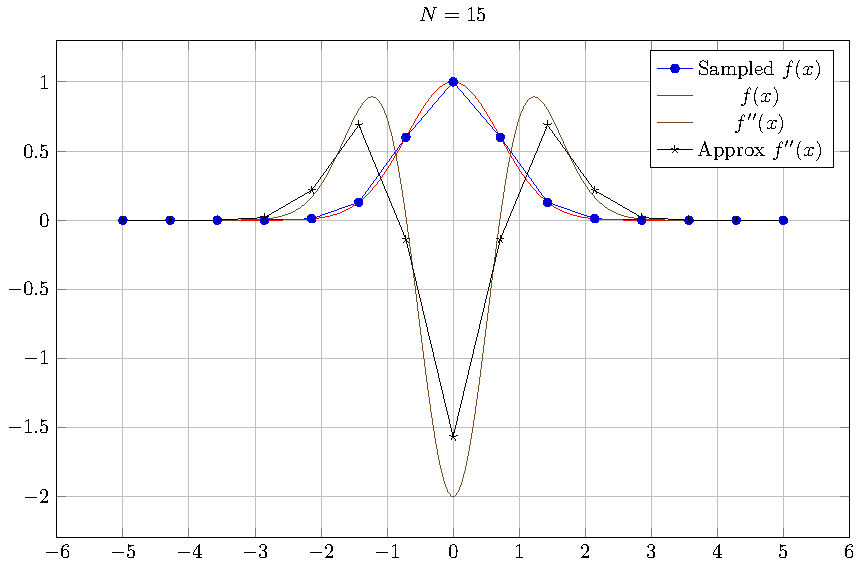
\includegraphics[scale=0.65]{../codes/FD1d/IMG_gaussian_15.pdf}\,%
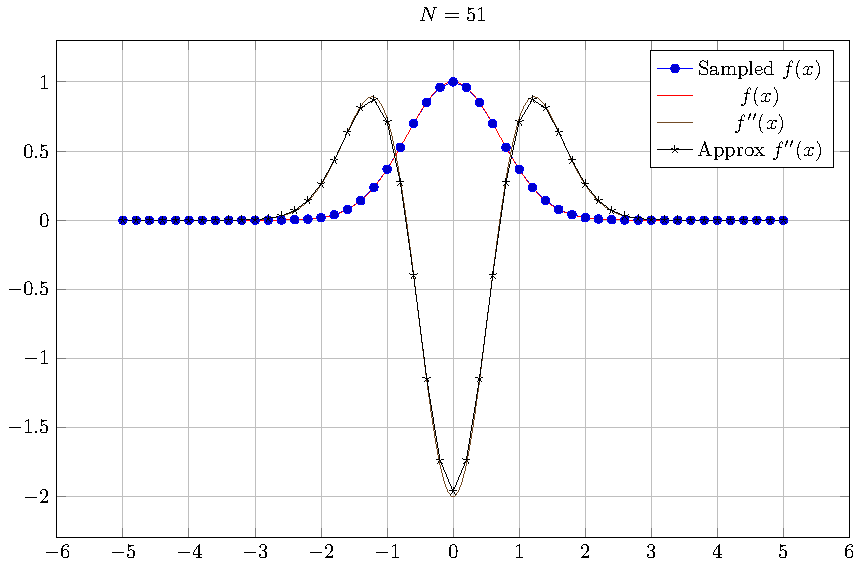
\includegraphics[scale=0.65]{../codes/FD1d/IMG_gaussian_51.pdf}
\par}
\caption{Finite difference approximation to a Gaussian function and its second derivative}
\label{fig:compare_2nd_deriv}
\end{figure}

In Figure \ref{fig:compare_2nd_deriv}, the comparison of analytical and numerical second derivative of
a Gaussian function is shown. It can be seen clearly that the accuracy of numerical second derivate
became better as the number of the grid points is increased.


\subsection{Harmonic potential}

Now that we know how to represent second derivative as a matrix, we are ready to solve the Schroedinger equation.
We will start with a simple potential $V(x)$ for which we know the exact solutions, i.e. the harmonic potential:
\begin{equation}
V(x) = \frac{1}{2}\omega^2 x^2
\end{equation}
where $\omega$ is a parameter.

The Hamiltonian in the finite difference representation takes the following form:
\begin{equation}
\mathbb{H} = -\frac{1}{2}\mathbb{D}^{(2)} + \mathbb{V}
\end{equation}
where $\mathbb{V}$ is a diagonal matrix whose elements are:
\begin{equation}
\mathbb{V}_{ij} = V(x_{i})\delta_{ij}
\end{equation}
and $\mathbb{D}^{(2)}$ is the second derivative matrix defined previously.

The following code calculates the harmonic potential with the default value
of $\omega=1$.
\begin{juliacode}
function pot_harmonic( x; ω=1.0 )
    return 0.5 * ω^2 * x^2
end
\end{juliacode}

The following Julia snippet illustrates the steps of constructing the Hamiltonian matrix,
starting from initialization of grid points, building the 2nd derivative matrix, and building
the potential.
\begin{juliacode}
# Initialize the grid points
xmin = -5.0; xmax = 5.0
N = 51
x, h = init_FD1d_grid(xmin, xmax, N)
# Build 2nd derivative matrix
D2 = build_D2_matrix_3pt(N, h)
# Potential
Vpot = pot_harmonic.(x)
# Hamiltonian
Ham = -0.5*D2 + diagm( 0 => Vpot )
\end{juliacode}

Once the Hamiltonian matrix has been constructed, we can find the solutions or the eigenvalues
and eigenvectors by solving the eigenproblem. In Julia, we can do this by calling the \txtinline{eigen}
function of \txtinline{LinearAlgebra} package which is part of the standard Julia library.
The following snippets shows how this can be achieved.
\begin{juliacode}
# Solve the eigenproblem
evals, evecs = eigen( Ham )
# We will show the 5 lowest eigenvalues
Nstates = 5
@printf("Eigenvalues\n")
for i in 1:Nstates
    @printf("%5d %18.10f\n", i, evals[i])
end
\end{juliacode}

We can compare our eigenvalues result with the analytical solution:
\begin{equation}
E_{n} = (2n - 1)\frac{\hbar}{2}\omega,\,\,\,n = 1,2,3,\ldots
\end{equation}
The results are shown in the following table for $N=51$.
\begin{table}[H]
{\centering
\begin{tabular}{|c|c|c|c|}
\hline
$n$ & Numerical & Exact & abs(error) \\
\hline
1   &    0.4987468513   &    0.5000000000  &   1.2531486828e-03 \\
2   &    1.4937215179   &    1.5000000000  &   6.2784821079e-03 \\
3   &    2.4836386480   &    2.5000000000  &   1.6361352013e-02 \\
4   &    3.4684589732   &    3.5000000000  &   3.1541026791e-02 \\
5   &    4.4481438504   &    4.5000000000  &   5.1856149551e-02 \\
\hline
\end{tabular}
\par}
\end{table}
You may try to vary the number of $N$ to achieve higher accuracy.

\begin{figure}[H]
{\center
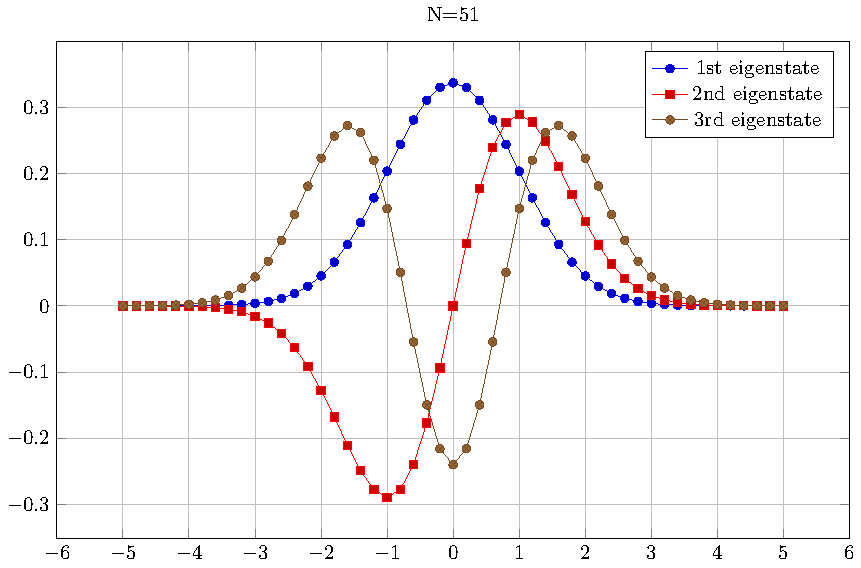
\includegraphics[scale=0.75]{../codes/sch_1d/IMG_main_harmonic_01_51.pdf}
\par}
\caption{Eigenstates of harmonic oscillator}
\label{fig:harm_eigenstates_N_51}
\end{figure}

In addition to the eigenvalues, we also can visualize the eigenfunctions or eigenstates. The results
are shown in Figure \ref{fig:harm_eigenstates_N_51} for $N=51$.

The full Julia program for this harmonic potential is given in \txtinline{sch_1d/main_harmonic_01.jl}.

Note that calling \txtinline{eigen} will give us $N$-pairs of eigenvalue-eigenfunctions where $N$ is the
dimension of the Hamiltonian matrix or in this case the number of grid points. We rarely needs all of these
eigenpairs.

\subsection{Higher order finite difference}

To achieve more accurate result we can include more points in our calculations. However there is an
alternative, namely by using more points or higher order formula to approximate second derivative
An example is 5-point formula for central difference approximation to second derivative:
\begin{equation}
\frac{\mathrm{d}^2}{\mathrm{d}x^2} \psi_{i} \approx
\frac{-\psi_{i+2} + 16\psi_{i+1} - 30\psi_{i} + 16\psi_{i-1} - \psi_{i-2}}{12h^2}
\end{equation}
%
The finite difference coefficients can be found in the literature or various sources on the web (for
example: \url{http://web.media.mit.edu/~crtaylor/calculator.html}).

We have provided Julia codes for calculating second derivative matrix using 5, 7, and 9 points
with the name \txtinline{build_D2_matrix_xpt.jl} where $x=5,7,9$.
You can repeat the calculation for harmonic oscillator potential with fixed number of $N$ and
and compare the eigenvalue results by using 3, 5, 7, and 9 points formula for second
derivative matrix.

%
%Eigenvalues
%    1       0.4999835358       0.5000000000   1.6464200292e-05
%    2       1.4998851344       1.5000000000   1.1486555438e-04
%    3       2.4995914414       2.5000000000   4.0855858565e-04
%    4       3.4989753444       3.5000000000   1.0246556283e-03
%    5       4.4979143167       4.5000000000   2.0856832921e-03
%efefer@mariya0704:~/.../sch_1d$ julia main_harmonic_02.jl 
%Eigenvalues
%    1       0.4999996353       0.5000000000   3.6467477399e-07
%    2       1.4999967387       1.5000000000   3.2613118246e-06
%    3       2.4999852653       2.5000000000   1.4734652533e-05
%    4       3.4999542324       3.5000000000   4.5767638893e-05
%    5       4.4998893996       4.5000000000   1.1060036071e-04
%efefer@mariya0704:~/.../sch_1d$ julia main_harmonic_02.jl 
%Eigenvalues
%    1       0.4999999886       0.5000000000   1.1404640010e-08
%    2       1.4999998762       1.5000000000   1.2379932590e-07
%    3       2.4999993334       2.5000000000   6.6659066622e-07
%    4       3.4999977023       3.5000000000   2.2976599006e-06
%    5       4.4999954715       4.5000000000   4.5284748360e-06